\documentclass[10pt]{article}
\usepackage[margin=0.9in]{geometry}


\usepackage{amsmath,amssymb}
\usepackage{booktabs}
\usepackage{tabularx}
\usepackage{array}
\usepackage{enumitem}
\usepackage{xcolor}
\usepackage{tikz}
\usetikzlibrary{positioning,arrows.meta,fit}
\usepackage[colorlinks=true,linkcolor=blue!50!black,urlcolor=blue!50!black,citecolor=blue!50!black]{hyperref}

\setlist{nosep,leftmargin=*}
\newcolumntype{L}{>{\raggedright\arraybackslash}X}
\newcommand{\status}[1]{\textsf{\small[#1]}}
\newcommand{\E}{\mathbb{E}}

\title{Options Pricing Through Generative Market Simulation\\[2pt]
\large Plan of action: which generative families to test, and how}
\author{ECE 6257 Final Project \quad Michael Incorvaia, Kian Chakamian, Rajan Sandhu, Yosep Rhe}
\date{Draft, October 25, 2026}

\begin{document}
\maketitle

\begin{abstract}
We compare generative model families as option pricers on a shared benchmark with exact ground truth.
The primary thesis is that discrete-token autoregressive (AR) models misprice deep out-of-the-money (OTM)
options and straddles because tokenization rounds extreme returns too coarsely, and that an AR transformer with a
continuous diffusion head fixes this at similar compute. Around that thesis we test MADE/RNADE, GANs, neural SDEs,
energy-based models, neural processes, VAEs and normalizing flows. Models split into two tracks:
\emph{market simulators} that learn from return histories and price by Monte Carlo (Track A), and
\emph{option-implied models} that learn from option quotes (Track B). Every model reports into one evaluation
harness, so results are directly comparable.
\end{abstract}

\section{Big picture}

\begin{figure}[h]
\centering
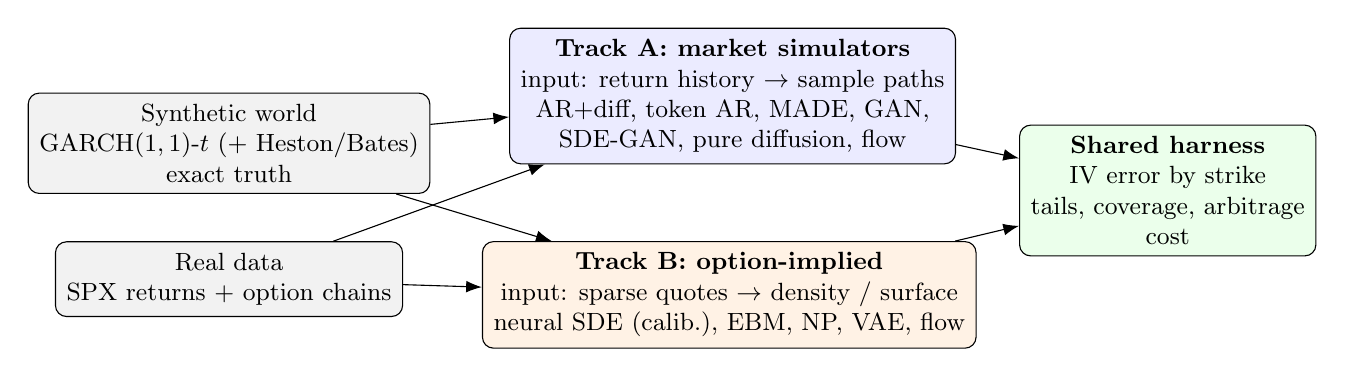
\begin{tikzpicture}[node distance=6mm and 10mm, font=\small,
  box/.style={draw, rounded corners, align=center, inner sep=4pt, minimum height=8mm},
  arr/.style={-{Latex[length=2mm]}}]
\node[box, fill=gray!10] (sim) {Synthetic world\\GARCH($1,1$)-$t$ (+ Heston/Bates)\\exact truth};
\node[box, fill=gray!10, below=of sim] (real) {Real data\\SPX returns + option chains};
\node[box, fill=blue!8, right=10mm of sim, yshift=6mm] (A) {\textbf{Track A: market simulators}\\input: return history $\to$ sample paths\\AR+diff, token AR, MADE, GAN,\\SDE-GAN, pure diffusion, flow};
\node[box, fill=orange!10, right=10mm of real, yshift=-2mm] (B) {\textbf{Track B: option-implied}\\input: sparse quotes $\to$ density / surface\\neural SDE (calib.), EBM, NP, VAE, flow};
\node[box, fill=green!8, right=8mm of A, yshift=-12mm] (H) {\textbf{Shared harness}\\IV error by strike\\tails, coverage, arbitrage\\cost};
\draw[arr] (sim) -- (A); \draw[arr] (sim) -- (B); \draw[arr] (real) -- (A); \draw[arr] (real) -- (B);
\draw[arr] (A) -- (H); \draw[arr] (B) -- (H);
\end{tikzpicture}
\caption{Two tracks, one ground truth, one harness.}
\end{figure}

\paragraph{Why two tracks.} Families generate different objects. A return-path simulator learns the
real-world measure $P$ from history; an option-implied model learns the pricing measure $Q$ from quotes.
Comparing them on one leaderboard would mix two questions. On synthetic data we price under the simulator's
own measure with $r=0$, so $P=Q$ and Track A has an exact answer; Track B gets exact answers because the true
surfaces come from the same simulator.

\paragraph{Paper scope.} A 4 to 6 page paper cannot hold nine model families in depth. The main paper is Track A
(the thesis) plus one headline Track B result; everything else goes in a results table and the appendix.
Section~\ref{sec:priorities} ranks what is required versus a stretch goal.

\section{Ground truth and data}

\subsection{D1: synthetic return paths (built)}
Daily log returns follow GARCH($1,1$) with standardized Student-$t$ shocks,
\[
r_t=\sigma_t\varepsilon_t,\qquad \sigma_{t+1}^2=\omega+\alpha r_t^2+\beta\sigma_t^2,\qquad
\varepsilon_t\sim t_\nu/\sqrt{\nu/(\nu-2)},
\]
with $\alpha=0.08$, $\beta=0.90$, $\nu=5$, 20\% long-run vol. A context window of $L=64$ days fixes the state
$\sigma^2_{L+1}$, so the true price of any payoff over the next $H=20$ days is computed by large Monte Carlo
from that state. Already implemented in \texttt{ardiff/data.py}.

\subsection{D2: synthetic option surfaces (to build)}
From D1 states, compute true prices on a grid of maturities $\tau\in\{5,10,20,40,60\}$ days and strikes
$K=S_0e^{k\,\mathrm{sd}_\tau}$, $k\in[-4,4]$, and convert to implied vol. Add a Heston/Bates family for variety
and as a case where the Heston baseline is \emph{correctly} specified. Quotes for Track B are drawn by
\begin{itemize}
\item \textbf{sparsity masks}: keep 5, 10 or 20 quotes; separate masks that drop the wings ($|k|>2$);
\item \textbf{noise}: bid/ask half-spread proportional to vega, plus occasional stale quotes.
\end{itemize}

\subsection{D3: real data}
\begin{itemize}
\item \textbf{Returns}: SPX (and a few single names) daily history, free sources.
\item \textbf{Options}: OptionMetrics IvyDB via WRDS if Georgia Tech access works; otherwise a limited free
end-of-day snapshot set collected over the project period.
\item \textbf{Caveat}: on real data Track A learns $P$ but market prices are $Q$, so comparing simulated prices to
market prices measures the variance risk premium, not model error. Real-data Track A is therefore evaluated by
\emph{backtest}: the model's predicted expected payoff should match the average realized payoff (and terminal
returns should be calibrated, measured by CRPS and PIT histograms).
\end{itemize}

\section{Shared harness}

\subsection{Interface (framework agnostic)}
Teammates work in PyTorch and JAX, so models talk to the harness through files, not code.
\begin{itemize}
\item \textbf{Track A}: read the fixed evaluation contexts \texttt{eval\_ctx.npy} $[E,L]$; write
\texttt{samples.npy} $[E,N,H]$ of future log returns (daily units) plus \texttt{meta.json}
(params, training GPU-hours, sampling seconds). The harness prices everything.
\item \textbf{Track B}: read \texttt{quotes.npz} (observed $(k,\tau,\sigma_{\text{imp}})$ per surface); write
predicted IVs at query points, optional 5/50/95\% bands, and, where the model has one, the density on a fixed
log-strike grid.
\end{itemize}
The current \texttt{ardiff/evaluate.py} already does the Track A pricing; the plan is to factor it into
\texttt{bench/} so it accepts any \texttt{samples.npy}.

\subsection{Metrics}
\begin{table}[h]
\centering\small
\begin{tabularx}{\linewidth}{@{}l L L@{}}
\toprule
& \textbf{Track A (simulators)} & \textbf{Track B (option-implied)} \\
\midrule
Pricing & mean $|$IV error$|$ by strike bucket: ATM ($|k|\le1$), wings ($2\le|k|\le4$); straddle error; stressed contexts (top third of state vol) reported separately
& IV RMSE on held-out quotes, wings separate; exotic price error (Track B2)\\
Distribution & terminal-return quantile error at 0.1, 1, 99, 99.9\%; CRPS; tail index (Hill) of daily returns; ACF of $|r_t|$ (vol clustering)
& Wasserstein-1 / KL between predicted and true risk-neutral density \\
Uncertainty & spread of prices across seeds and sample sets
& coverage of 90\% bands; CRPS \\
Validity & rate of explosive samples (step $>50$ std)
& static-arbitrage violations (butterfly, calendar)\\
Cost & params; training GPU-hours; $\mu$s per generated path
& fit or inference time per surface\\
\bottomrule
\end{tabularx}
\caption{One metric set per track. IV error is the headline because it compares deep OTM fairly, where raw prices are tiny.}
\end{table}

\section{Track A: market simulators}

Each card lists the hypothesis, the setup, the key experiments and the main risk.

\subsection{A1. AR transformer + diffusion head (ours) \status{built, v0 ready to run}}
\begin{itemize}
\item \textbf{Model}: causal transformer over continuous returns; a small AdaLN-MLP DDPM head generates each next
return with no quantization (MAR-style \cite{mar}). JAX/Flax, \texttt{ardiff/}.
\item \textbf{Hypothesis H1}: wing IV error ($|k|\ge2$) is lower than the token AR at matched backbone and similar
cost; the gap grows in stressed contexts and with heavier tails (smaller $\nu$).
\item \textbf{Experiments}: v0 comparison (\texttt{scripts/run\_thesis\_v0.sh}); ablations over sampling steps
(cost vs accuracy curve), head width, $\nu\in\{3,5,8\}$, and a \textbf{flow-matching head} in place of DDPM.
\item \textbf{Risk}: rare explosive samples fed back autoregressively (seen once in the smoke test). Track the
explosive-sample rate; do not clip, since clipping is exactly the failure being studied.
\end{itemize}

\subsection{A2. Tokenized AR (Kronos-style) \status{built}}
\begin{itemize}
\item Same backbone, softmax over return bins. Variants: 256 quantile bins, 1024 uniform bins clipped at $\pm8$ std;
decode to bin mean (default), center, or jitter.
\item \textbf{Fairness rules}: report the decode mode; sweep $n_{\text{bins}}\in\{64,\dots,4096\}$ so the claim is
not ``tokens lose because we picked too few.''
\item \textbf{Stretch}: pretrained Kronos \cite{kronos} itself on real data.
\end{itemize}

\subsection{A3. MADE / RNADE \status{teammate, in progress}}
\begin{itemize}
\item \textbf{Model}: autoregressive density over a fixed window with Gaussian-mixture conditionals (RNADE) or
masked MLP (MADE) \cite{made,rnade}.
\item \textbf{Conditioning tip}: put the $L$ context days as the first $L$ dimensions of the ordering, train on
$L+H$ windows, and sample only the last $H$ dimensions with the first $L$ clamped to the context. No architecture
change needed.
\item \textbf{Hypothesis H2}: a mixture output is continuous, so tails should beat the token AR; but with no
attention over long history it should trail A1 when conditioning on the vol state matters (stressed contexts).
\item \textbf{To check}: the current notebook's toy data repeats one move across all steps; switch to D1.
\end{itemize}

\subsection{A4. GAN \status{teammate, in progress}}
\begin{itemize}
\item \textbf{Model}: conditional time-series GAN, e.g.\ Quant GAN (TCN generator) \cite{quantgan} or a
signature-Wasserstein GAN.
\item \textbf{Hypothesis H3}: GANs match bulk statistics but under-cover the tails (mode dropping), so wing IV
error and 99.9\% quantile error are worse than A1 even when the discriminator score looks good. This doubles as a
``generative metrics vs pricing metrics'' result.
\item \textbf{Risk}: training instability; report several seeds.
\end{itemize}

\subsection{A5. Neural SDE as a GAN (Kidger et al.) \status{to build}}
\begin{itemize}
\item \textbf{Model}: $dX_t=\mu_\theta(t,X_t,c)\,dt+\sigma_\theta(t,X_t,c)\,dW_t$ with context embedding $c$,
trained adversarially with a neural CDE discriminator \cite{kidger}. JAX: \texttt{diffrax}.
\item \textbf{Hypothesis H4}: continuous-time structure gives stable, well-behaved paths (no explosive samples) and
good vol clustering, but Brownian driving noise underweights jumps, so extreme wings ($|k|=4$) trail A1.
\item \textbf{Variant}: add a jump component (L\'evy driving noise) as an ablation, since that is the obvious fix.
\end{itemize}

\subsection{A6. Pure diffusion, no time structure \status{to build}}
\begin{itemize}
\item \textbf{Model}: one DDPM over the whole $H$-day future vector, conditioned on a context summary (MLP or the A1
backbone's final state).
\item \textbf{Hypothesis H5}: matches A1 on terminal-return quantiles (so on vanilla prices) but loses on
path-dependent payoffs and vol clustering, which isolates what the AR structure buys.
\end{itemize}

\subsection{A7. Conditional normalizing flow \status{to build}}
\begin{itemize}
\item \textbf{Model}: neural spline flow \cite{nsf} over the $H$-day future given the context; exact likelihood,
one-shot sampling. JAX: \texttt{flowjax} or a small hand-written RealNVP/spline flow.
\item \textbf{Role}: the fast baseline. Gives held-out log-likelihood, which A2/A3/A7 can be compared on directly.
\item \textbf{Hypothesis H6}: competitive on vanillas at a small fraction of A1's sampling cost; tails are limited
by the Gaussian base distribution unless a heavy-tailed base ($t$ base) is used, which is a clean ablation.
\end{itemize}

\section{Track B: option-implied models}

Track B has three tasks: \textbf{B1} recover the risk-neutral density at one maturity from sparse quotes;
\textbf{B2} calibrate to vanillas and price exotics; \textbf{B3} complete a whole surface from scattered quotes.

\subsection{B-baselines (needed for every Track B claim)}
SVI/SSVI fits \cite{ssvi}, cubic spline on IV, Breeden-Litzenberger with smoothing, mixture of lognormals, a
Gaussian process on IV, classical max-entropy \cite{buchenkelly}, and Heston calibration.

\subsection{B1/B2. Neural SDE calibrated to options (Gierjatowicz et al.) \status{to build}}
\begin{itemize}
\item \textbf{Model}: fix the drift at $r$ (risk-neutral by construction), learn $\sigma_\theta(t,S_t,V_t)$ so
Monte Carlo prices match observed vanillas \cite{neuralsde}. Ensembles or the paper's robust bounds give a price
band for exotics. JAX: \texttt{diffrax}, differentiate through the Monte Carlo.
\item \textbf{Hypothesis H7}: on D2 surfaces where Heston is misspecified (GARCH-$t$ truth), both fit vanillas, but
for exotics (barrier, Asian, lookback, forward-start straddle) the neural SDE's error is lower and its band covers
the true price far more often than Heston's point estimate. On Heston-generated surfaces, Heston should win; that
is the control.
\end{itemize}

\subsection{B1. Energy-based model / maximum entropy \status{to build}}
\begin{itemize}
\item \textbf{Classical}: the max-entropy density matching quotes $\{c_i\}$ is
$p(x)\propto\exp\!\big(-\sum_i\lambda_i (e^x-K_i)^+\big)$ times a prior \cite{buchenkelly}, already an EBM.
\item \textbf{Neural}: $E_\theta(x)=\sum_i\lambda_i\,\text{payoff}_i(x)+g_\theta(x)$, or an amortized network that
maps a quote set to $E$, trained across many D2 surfaces. Price constraints enforced by penalty or Lagrangian.
\item \textbf{Sampling}: in 1-D the normalizer is computed exactly by quadrature on a grid; Langevin is needed only
for the joint multi-maturity version (stretch).
\item \textbf{Hypothesis H8}: with 5 to 10 quotes, the amortized EBM recovers the density (Wasserstein-1) and the
missing wings better than classical max-entropy and SVI, because it has learned what plausible densities look
like. A valid density is free of within-maturity static arbitrage by construction.
\end{itemize}

\subsection{B3. Neural process \status{to build}}
\begin{itemize}
\item \textbf{Model}: (attentive) neural process \cite{np,anp}; context set = observed $(k,\tau,\sigma_{\text{imp}})$,
target = full surface with predictive mean and variance. The encoder is a permutation-invariant set function
(DeepSets), which is the geometric-DL tie-in.
\item \textbf{Hypothesis H9}: lower held-out IV RMSE than SVI/spline/GP when quotes are sparse or wings are missing,
\emph{and} calibrated 90\% bands (coverage near 90\%). Calibration is the selling point; RMSE alone is not.
\item \textbf{Risk}: needs many training surfaces; D2 provides unlimited synthetic ones, so test sim-to-real
transfer on D3.
\end{itemize}

\subsection{B3. VAE on vol surfaces \status{to build}}
\begin{itemize}
\item \textbf{Model}: VAE on gridded surfaces with a 2 to 4 dimensional latent \cite{bergeron,ning}; completion by
optimizing the latent to fit sparse quotes (Bergeron et al.).
\item \textbf{Hypothesis H10}: latents line up with trader factors; measure $R^2$ of each latent against level,
skew and term-structure slope (and against the true GARCH state on D2). Walking a latent produces realistic,
arbitrage-free surface moves for stress tests (check the violation rate).
\item \textbf{Comparison}: also run as a completion method head-to-head with the neural process.
\end{itemize}

\subsection{B1. Normalizing flow for the risk-neutral density \status{to build}}
\begin{itemize}
\item 1-D flow density per maturity, fitted so its expected payoffs match quotes (reparameterized Monte Carlo or
quadrature). A smooth, positive density with exact likelihood; the simplest neural baseline for B1 against the EBM.
\end{itemize}

\section{Hypotheses at a glance}
\begin{table}[h]
\centering\small
\begin{tabularx}{\linewidth}{@{}l L l@{}}
\toprule
& \textbf{Claim (falsifiable)} & \textbf{Main metric}\\
\midrule
H1 & AR+diffusion beats token AR in the wings at similar cost & wing IV error, $\mu$s/path\\
H2 & MADE/RNADE beats token AR in tails, trails A1 in stressed contexts & stressed wing IV error\\
H3 & GAN under-covers tails despite good discriminator scores & 99.9\% quantile error\\
H4 & SDE-GAN is stable but underweights jumps & $|k|=4$ IV error, explosive rate\\
H5 & Pure diffusion matches A1 on vanillas, loses on path-dependent payoffs & exotic error, ACF of $|r|$\\
H6 & Flow is competitive on vanillas at a fraction of the cost & IV error vs $\mu$s/path\\
H7 & Calibrated neural SDE prices exotics better than Heston when Heston is wrong & exotic error, band coverage\\
H8 & Amortized EBM recovers densities from sparse quotes better than max-ent/SVI & $W_1$ to true density\\
H9 & Neural process completes surfaces with calibrated uncertainty & held-out RMSE, 90\% coverage\\
H10 & VAE latents match level/skew/term factors & $R^2$, arbitrage rate\\
\bottomrule
\end{tabularx}
\end{table}

\section{Priorities, owners and timeline}\label{sec:priorities}

\begin{table}[h]
\centering\small
\begin{tabularx}{\linewidth}{@{}l l l L@{}}
\toprule
\textbf{Tier} & \textbf{Item} & \textbf{Owner} & \textbf{Why}\\
\midrule
1 (required) & A1 AR+diffusion, A2 token AR & Michael & the thesis\\
1 & A3 MADE/RNADE & teammate & already in progress\\
1 & A4 GAN & teammate & already in progress\\
1 & Shared harness + D2 generator & TBD & everything depends on it\\
2 (strong) & A5 SDE-GAN, B2 calibrated neural SDE & TBD & best Track B headline; shares \texttt{diffrax} code\\
2 & A6 pure diffusion, A7 flow & TBD & cheap, sharpen the thesis\\
2 & B3 neural process & TBD & clean geometric-DL tie-in\\
3 (stretch) & B1 EBM, B1 flow, B3 VAE & TBD & appendix material\\
3 & Real data (D3), pretrained Kronos & TBD & external validity\\
\bottomrule
\end{tabularx}
\end{table}

\paragraph{Timeline (relative to the due date, to be fixed).}
\begin{enumerate}
\item \textbf{Week 1}: factor the harness into \texttt{bench/} with the \texttt{.npy} interface; publish the
fixed evaluation contexts; build D2; port MADE and GAN onto D1; launch the A1/A2 v0 runs on PACE.
\item \textbf{Week 2}: first Track A leaderboard (A1 to A4); start A5 and B2 (shared neural SDE code).
\item \textbf{Week 3}: A6, A7; B3 neural process; Track B baselines.
\item \textbf{Week 4}: ablations for H1 ($n_{\text{bins}}$, sampling steps, $\nu$, flow-matching head); B2 exotics;
first real-data pass.
\item \textbf{Week 5}: tier 3 as time allows; seeds and error bars; freeze results.
\item \textbf{Week 6}: write the paper (ICML style, 4 to 6 pages), figures, appendix.
\end{enumerate}

\paragraph{Conventions.} Fixed seeds and data splits in config; every run writes its config and git hash next to
its results; one results table generated from \texttt{results/*.json}, never by hand.

\section{Related work to read first}
Three recent papers apply diffusion to implied-vol surfaces \cite{ivdiff1,ivdiff2,ivdiff3}; check that none
already does an AR + continuous head for path generation before claiming novelty.

\begin{thebibliography}{99}\small
\bibitem{mar} T.~Li et al., Autoregressive image generation without vector quantization, NeurIPS 2024, arXiv:2406.11838.
\bibitem{kronos} Kronos: a foundation model for the language of financial markets, arXiv:2508.02739.
\bibitem{made} M.~Germain et al., MADE: masked autoencoder for distribution estimation, ICML 2015.
\bibitem{rnade} B.~Uria, I.~Murray, H.~Larochelle, RNADE: the real-valued neural autoregressive density-estimator, NeurIPS 2013.
\bibitem{quantgan} M.~Wiese et al., Quant GANs: deep generation of financial time series, Quantitative Finance, 2020.
\bibitem{kidger} P.~Kidger et al., Neural SDEs as infinite-dimensional GANs, ICML 2021.
\bibitem{neuralsde} P.~Gierjatowicz et al., Robust pricing and hedging via neural SDEs.
\bibitem{nsf} C.~Durkan et al., Neural spline flows, NeurIPS 2019.
\bibitem{buchenkelly} P.~Buchen, M.~Kelly, The maximum entropy distribution of an asset inferred from option prices, JFQA, 1996.
\bibitem{np} M.~Garnelo et al., Neural processes, 2018.
\bibitem{anp} H.~Kim et al., Attentive neural processes, ICLR 2019.
\bibitem{bergeron} M.~Bergeron et al., Variational autoencoders: a hands-off approach to volatility.
\bibitem{ning} B.~Ning, S.~Jaimungal, X.~Zhang, M.~Bergeron, Arbitrage-free implied volatility surface generation with variational autoencoders.
\bibitem{ssvi} J.~Gatheral, A.~Jacquier, Arbitrage-free SVI volatility surfaces, Quantitative Finance, 2014.
\bibitem{ivdiff1} Forecasting implied volatility surface with generative diffusion models, arXiv:2511.07571.
\bibitem{ivdiff2} Arbitrage-aware multi-step forecasting of implied volatility surfaces using latent diffusion, arXiv:2608.22478.
\bibitem{ivdiff3} Diffusion models for dynamic volatility surface generation and data-driven hedging, arXiv:2609.13402.
\end{thebibliography}

\end{document}
